Fortsetter fra forrige kapittel.

Avhengig av forholdet mellom $A \cdot \beta$ vil signalet endre seg
på forskjellig måte.

\paragraph{Loopgain $< 1$} \mbox{} \\
\begin{figure}[H]
  \caption{Oscillasjon dør ut}
  \centering
  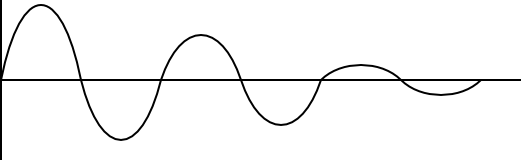
\includegraphics[width=0.5\textwidth]{./img/fadingsignal}
\end{figure}

\paragraph{Loopgain $> 1$} \mbox{} \\
\begin{figure}[H]
  \caption{Signalet øker til clipping}
  \centering
  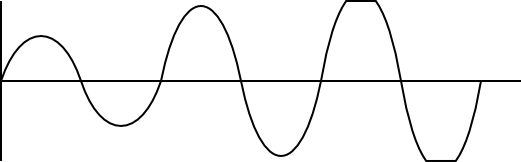
\includegraphics[width=0.5\textwidth]{./img/gainingsignal}
\end{figure}

\paragraph{Loopgain $= 1$} \mbox{} \\
\begin{figure}[H]
  \caption{Stabilt signal}
  \centering
  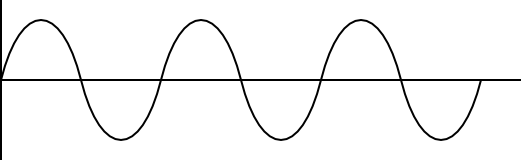
\includegraphics[width=0.5\textwidth]{./img/stabiltsignal}
\end{figure}
